%!TEX root = main_ISMB.tex
\section{Supplementary data}
\subsection{RNAinverse}
Using the same dataset of $50$ structures, we generated $100$ samples
per structure with \RNAinverse. They yield for most parameters
a high entropy. For all structures that have been solved 
by the three methods, only \RNAinverse, only \texttt{Incarnation} and
\texttt{Incarnation} followed by \RNAinverse,
we present for every different concentration of \texttt{C+G}
the average sample entropy and the average base pairs entropy.


\begin{figure}[ht!]
	\centering
	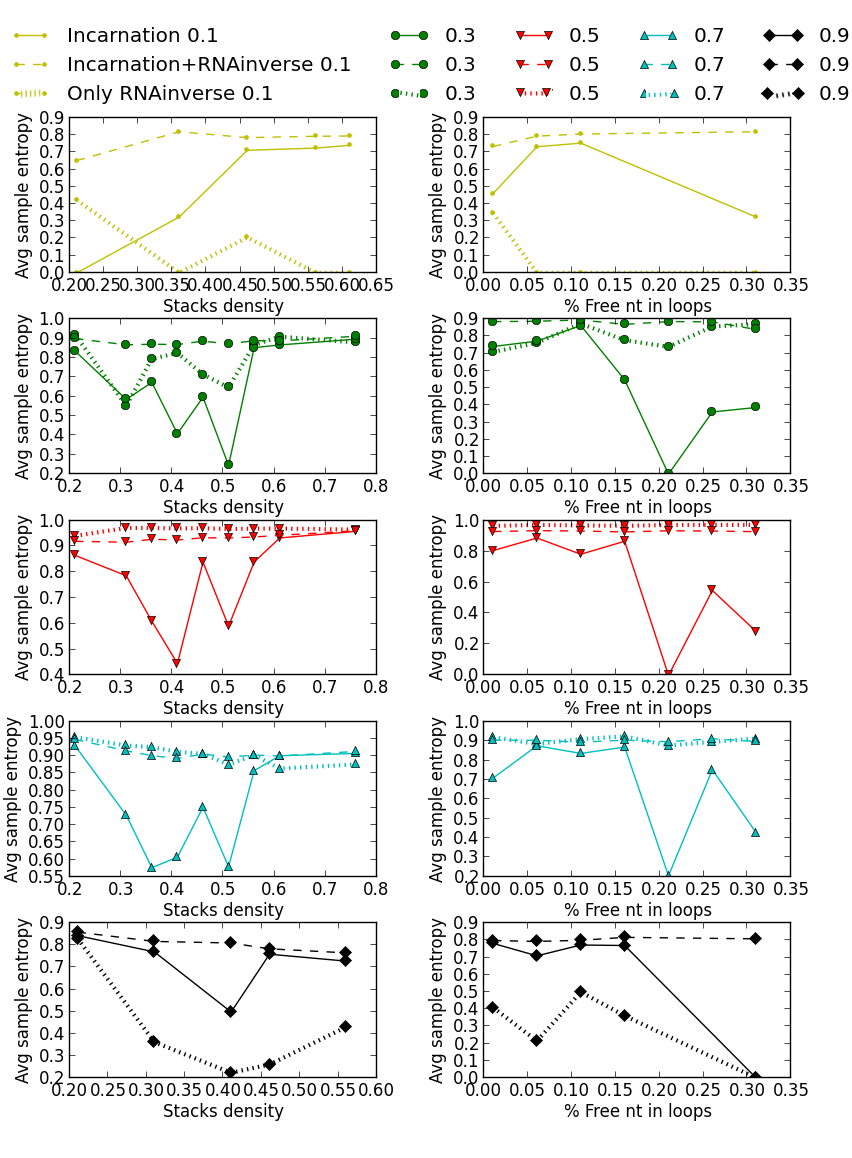
\includegraphics[scale=0.4]{Figures/RNAinverse_data_100.png}
	\caption{Entropy and \texttt{C+G} content for structures solved by
	the 3 methods.}
	\label{fig:rnainverse}
\end{figure}

%The same analysis but only for structures solved by \texttt{Incarnation}
%and \texttt{Incarnation} followed by \RNAinverse, is presented in 
%Fig.~\ref{fig:inc_rnainv}
%
%\begin{figure}
%	\centering
%	\includegraphics{}
%	\caption{Entropy and \texttt{C+G} content for structures solved by
%	the \texttt{Incarnation} and \texttt{Incarnation}$+$\RNAinverse.}
%	\label{fig:inc_rnainv}
%\end{figure}